  %%%%%%%%%%%%%%%%%%%%%%%%%%%%%%%%%%%%%%%%%%%%%%%%%%%%%%%%%%%%%%%%%%%%%%
% LaTeX Example: Project Report

%%% Preamble
\documentclass[paper=a4, fontsize=11pt, abstract=on]{scrartcl}
\usepackage[T1]{fontenc}
\usepackage{fourier}
\usepackage{tabularx}
\usepackage[utf8]{inputenc}
\usepackage{hyperref}





\usepackage{listings}
\usepackage{color}

\definecolor{dkgreen}{rgb}{0,0.6,0}
\definecolor{gray}{rgb}{0.5,0.5,0.5}
\definecolor{mauve}{rgb}{0.58,0,0.82}
\lstset{frame=tb,
  language=[Visual]C++,
  aboveskip=3mm,
  belowskip=3mm,
  showstringspaces=false,
  columns=flexible,
  basicstyle={\small\ttfamily},
  numbers=none,
  numberstyle=\tiny\color{gray},
  keywordstyle=\color{blue},
  commentstyle=\color{dkgreen},
  stringstyle=\color{mauve},
  breaklines=true,
  breakatwhitespace=true,
  tabsize=3
}
\usepackage{graphicx}
\usepackage{caption}
\usepackage{subcaption}

\usepackage[english]{babel}															% English language/hyphenation
\usepackage[protrusion=true,expansion=true]{microtype}	
\usepackage{amsmath,amsfonts,amsthm} % Math packages

\usepackage{url}
%\usepackage[hang, small,labelfont=bf,up,textfont=it,up]{caption}


%%% Custom sectioning
\usepackage{sectsty}
\allsectionsfont{\normalfont\scshape}
\usepackage{float}
\usepackage{amsmath}
\usepackage{mathtools}
\usepackage{ragged2e}

\usepackage{nomencl}
\makenomenclature

%%% Custom headers/footers (fancyhdr package)
\usepackage{fancyhdr}
\pagestyle{fancyplain}
\fancyhead{}											% No page header
\fancyfoot[L]{}											% Empty 
\fancyfoot[C]{}											% Empty
\fancyfoot[R]{\thepage}									% Pagenumbering
\renewcommand{\headrulewidth}{0pt}			% Remove header underlines
\renewcommand{\footrulewidth}{0pt}				% Remove footer underlines
\setlength{\headheight}{13.6pt}
   \renewcommand*\abstractname{Summary}

%%% Equation and float numbering
\numberwithin{equation}{section}		% Equationnumbering: section.eq#
\numberwithin{figure}{section}			% Figurenumbering: section.fig#
\numberwithin{table}{section}				% Tablenumbering: section.tab#


%%% Maketitle metadata

\newcommand{\horrule}[1]{\rule{\linewidth}{#1}} 	% Horizontal rule

\title{
		%\vspace{-1in} 	
		\usefont{OT1}{bch}{b}{n}
		\normalfont \normalsize \textsc{} \\ [25pt]
		
\includegraphics[width=0.3\linewidth]{ubc.png} \\
		%
\includegraphics[width=0.4\linewidth]{tru}		
		\horrule{0.5pt} \\[0.2cm]
		\huge Programming Assignment \#2 : Solving 1D Wave Equation  \\
		\horrule{2pt} \\[0.005cm]
}
\author{
		\normalfont 								\normalsize
        Jerin Roberts\\[-5pt]		\normalsize
        \today
}
\date{}




%%% Begin document
\begin{document}
\maketitle
\begin{center}
\begin{tabular}{l r}


Supervisor: & Dr. Carl Ollivier-Gooch  \\ % supervisor
Locations: & University of British Columbia


\end{tabular}
\end{center}



\newpage
\tableofcontents
\listoffigures
\listoftables
\newpage
\lstset{language=[Visual]C++}
\section{Overview}



 The are many physical phenomenons in physics and engineering that require linear and non-linear partial differential equations to described the true nature of the system. Solving these systems analytically and finding exact solutions for these equations can be difficult and often require simplifications that ultimately don't fully represent the problem being investigated. Numerical methods for solving PDE's provides a means for finding approximations to the exact solutions without having to make sacrificial simplifications. With recent advancements in computational technology numerical methods can now be easily applied to large and difficult problems that would otherwise be impossible to solve. 
\subsection{Theory}
Numerical problems are essentially solved by breaking the entire solution domain into small discrete points (mesh) and finding the solution at or around these areas. Each point requires the solving the differential equations that represent physical phenomenon being investigated. Since the exact solution cannot be computed, it is instead approximated using various techniques and methods. 

The Runge-Kutta scheme is a family of numerical techniques used to solve ordinary differential equations by numerically integrating using trial steps at the midpoints of an interval to cancel out lower-order error terms. A two stage Runge-Kutta scheme is displayed in equation \ref{rung2} which uses Explicit Euler as the first intermediate step \ref{rung1}.
 

 \begin{equation}
\label{rung1}
w^{(1)}=w^n+\triangle t(\lambda w^n)
\end{equation} 


 \begin{equation}
\label{rung2}
w^{n+1}=w^n+\triangle t\Bigg(\frac{\lambda w^n+\lambda w^{(1)}}{2}\Bigg)
\end{equation}

 The program will implement a 2nd order up wind flux evaluation method and a two-stage Runge-Kutta time advance scheme. For each interior volume cell the net flux will be calculated for a specific time step using the second order up wind method. The flux for the face $i=3/2$ is displayed in equation \ref{fl}. The flux is evaluated at each face and then the faces surrounding a single cell are summed to find the flux through that cell. Integrating this into equation \ref{wave} the wave equation can be evaluated using equation \ref{th}
 
  \begin{equation}
\label{wave}
\frac{\partial T}{\partial t} + u\frac{\partial T}{\partial x} = 0
\end{equation}

 \begin{equation}
\label{fl}
T_{\frac{3}{2}}=\frac{3\overline{T}_{1}-\overline{T}_{0}}{2} 
\end{equation}

 \begin{equation}
\label{th}
\frac{\partial T}{\partial t} + u\Bigg(\frac{3\overline{T}_{i}-4\overline{T}_{i-1}+\overline{T}_{i-2}}{2\triangle x}\Bigg)  = 0
\end{equation}

Boundary conditions will be implement using ghost cells allowing the interior scheme to remain the same during calculation of bordering cells. Because the interior scheme requires two upwind values, two ghost cells are required for this scheme to run on the first interior cell $i=1$. The ghost cells are calculated such the boundary condition is enforced at $i=1/2$. 



\begin{equation}
\label{neum}
\overline{T}_{0} = 2\overline{T}_{w}-\overline{T}_{1} 
\end{equation} 

\begin{equation}
\label{neum2}
\overline{T}_{-1} = -2\overline{T}_{w}+3\overline{T}_{0} 
\end{equation} 


The value for the ghost cells implementing Neumann Boundary at $x=0$ is calculated using equation \ref{neum} for cell $i = 0$ and \ref{neum2} for cell $i = -1$.
 


\section{Implementation}
\subsection{Program Overview}
The C/C++language was selected for this programming assignment. The scripts were compiled using g++/gcc version 5.4.0 on Ubuntu 16.04.02 and are available in the attached zip or for clone via the link provided: \url{https://github.com/j16out/cfd510} . The program itself is broken into 3 pieces and two levels to produce a modular set that makes it easier to apply to different problems. The highest level contains the "macro" or the main function which can be modified for different problems. 

\begin{table}[H]
\begin{center}
    \begin{tabular}{ | p{0.23\linewidth} | p{0.6\linewidth} |}
 \hline  
     \RaggedRight \textbf{Function}
    &\RaggedRight \textbf{Purpose}
    \\ \hline  
           \RaggedRight set\_ array\_ size() 
    &\RaggedRight Set size of array if not default(160x160)
    \\ \hline 
           \RaggedRight set\_ ghostcells()
    &\RaggedRight Set Ghost cells and update boundary conditions
    \\ \hline 
    \RaggedRight set\_ zero()
    &\RaggedRight Zero entire array including ghost cells
    \\ \hline 
           \RaggedRight set\_ intial\_ cond()
    &\RaggedRight Set initial condition
    \\ \hline 
           \RaggedRight print\_ array()
    &\RaggedRight Prints array in terminal style output
    \\ \hline 
           \RaggedRight get\_ FIarray()
    &\RaggedRight Evaluates Flux for array interior cells
    \\ \hline 
           \RaggedRight get\_ RK2()
    &\RaggedRight performs RK2 iteration 1 or 2 stage
    \\ \hline 
      \RaggedRight get\_ FIarray\_ 1stcell()
    &\RaggedRight Calculates flux at 1st interior cell
    \\ \hline 
    \RaggedRight  get\_ surcells()
    &\RaggedRight Gets current solution of neighboring cells
    \\ \hline 
    \RaggedRight  mv\_ SOL2\_ to\_ SOL1()
    &\RaggedRight moves updated solution to first stage array
    \\ \hline 
    \RaggedRight  solve\_ arrayRK2()
    &\RaggedRight Performs are steps to solve problem
    \\ \hline 
    \RaggedRight get\_ l1norm()
    &\RaggedRight Returns $L^1$ norm error
      \\ \hline 
    \RaggedRight get\_ l2norm()
    &\RaggedRight Returns $L^2$ norm error between two arrays of equal size
    \\ \hline 
    \RaggedRight get\_ linf\_ norm() 
    &\RaggedRight Returns $L^{\infty}$ norm error between two arrays of equal size
    \\ \hline 
    \RaggedRight set\_ analytic() 
    &\RaggedRight Set array values to predefined exact solution
    \\ \hline 
   
   
    
    \end{tabular}
\end{center} 
\caption{List of Program Functions}
\label{func} 
\end{table}

The numerical directory contains numerical.cpp script and its header file numerical.hpp. This set contains all the functions necessary for solving the problem numerically. Table \ref{func} displays all functions with a short description of each. The vroot directory contains the scripts necessary for drawing data. These scripts make use of the ROOT-v6 libraries. ROOT is a popular data analysis framework primarily written in C++ and Phython. For more information on ROOT libraries visit the link provided: \url{https://root.cern.ch/} .
The functions act on a structure called $carray$ which contains the solution domain array and its various parameters. The struct contains the main array, its defined working area (mesh size), data storage vectors, iteration count, and the represented dimension between points. Having these organized in a struct provides a compact way of passing and modifying the array and all its pertinent parameters. The outline of the struct used for the wave equation problem is shown below.


\begin{lstlisting}
struct carray{
//arrays
float mcellSOL [maxx][maxy];//first stage and solution mesh
float mcellSOL2 [maxx][maxy];//second stage solution mesh
float mcellFI [maxx][maxy];//first stage flux
float mcellFI2 [maxx][maxy];//second stage flux

//array attributes
int sizex = maxx;
int sizey = maxy;
float DIM1 = 0;

//current time 
float tstep = 0;
float ctime = 0;

//temporary cells to store
float Tim1_j=0.0;
float Tim2_j=0.0;
float Ti_j=0.0;

};
\end{lstlisting}
 
\subsection{1D Wave Problem}
The program was used to solve and find solutions to the 1D wave equation with information moving left to right (\ref{sim}) while satisfying conditions (\ref{con}). An exact solution to this problem is provided and written as $T(x,t)$ and displayed in equation \ref{ddd}. An exact solution will enabled a comparison against the numerical solution for error assessment. 

 \begin{equation}
\label{sim}
\frac{\partial T}{\partial t} + u\frac{\partial T}{\partial x} = 0
\end{equation}

 \begin{equation}
\label{con}
0\leq x \leq x_{max} \hspace{35pt} 0 \leq t \hspace{35pt} u = 2
\end{equation}

 \begin{equation}
\label{ddd}
T(x,t) = \sin{(2\pi (2t-x))}
\end{equation}

\subsection{Boundary Conditions}
Boundary Conditions are implemented through the calculation of the ghost cells. For the purely up wind scheme, we require two ghost cells to be calculated. The ghost cell is calculated such that the boundary is implemented at the face between the first ghost cell and first interior cell. Below shows the function that implements boundaries for the Wave problem.

\begin{lstlisting}
void set_ghostcells(carray & myarray)
{
float DIM1 = myarray.DIM1;
//set boundary conditions in ghost cells
if(myarray.scheme == 0)//2nd order upwind
{
myarray.mcellSOL2[0][1] = -2.0*(sin(4.0*PI*myarray.ctime)) + 3.0*myarray.mcellSOL[1][1];
myarray.mcellSOL2[1][1] = 2.0*(sin(4.0*PI*myarray.ctime)) - myarray.mcellSOL[2][1];
}

if(myarray.scheme == 1)//1st order upwind
{
myarray.mcellSOL2[1][1] = 2.0*(sin(4.0*PI*myarray.ctime)) - myarray.mcellSOL[2][1];
}

if(myarray.scheme == 2)//2nd order centered
{
myarray.mcellSOL2[1][1] = 2.0*(sin(4.0*PI*myarray.ctime)) - myarray.mcellSOL[2][1];
}

}
\end{lstlisting}
A loop is not necessary as this is purely a 1D problem therefore only two cells need to be updated each time step iteration. This subroutine will not need to be modified when the program is applied to different problems or using different flux schemes at the boundary as its switchable during run-time. Initial Conditions are set before the problem is solved using the subroutine shown below.
\begin{lstlisting}
void set_intial_cond(carray & myarray)
{
float DIM1 = myarray.DIM1;
float dx =0.0;
float f;
for(int j = 1; j < myarray.sizey-1; ++j)
{
    for(int i = 2; i < myarray.sizex; ++i)
    {
    dx = (i-1.5)*DIM1;
    f = -sin(2.0*PI*dx);
    myarray.mcellSOL[i][j] = f;
    }
}
}
\end{lstlisting}
The loop calculates all the values of T at time t=0 for varying x using equation \ref{int}. Unlike the boundary conditions the initial conditions are not modifiable during run-time and will need to be tailored to specific problems.

 \begin{equation}
\label{int}
T(x,0) = -\sin{(2\pi x)}
\end{equation}
  
\subsection{Iteration Scheme}
A RK2 routine was implemented to solve the system of equations approximating the solution at each grid point which is denoted as function $solve\_ arrayRK2$. The routine starts from the first interior cell $i = 2$ and iterates flux integration schemes until $i = i_{max}$. Once the flux values have been gathered for each face and expressed as a single cell value a subroutine calculates the time advance solution at each cell. Below shows both the flux calculating and solution calculating subroutines respectively.

\begin{lstlisting}
void get_FIarray(carray & myarray, int stage)
{
for(int j = 1; j < myarray.sizey-1; ++j)
{
    for(int i = 3; i < myarray.sizex; ++i)
    {
    //----get surrounding cells and compute new cell-------//
    get_surcells(myarray, i, j, stage);
    float newcell = calc_2nd_UW(myarray); 
    //-----update current cell----//
    if(stage == 1)
    myarray.mcellFI[i][j] = newcell;
    if(stage == 2)
    myarray.mcellFI2[i][j] = newcell;
    }
}
}
\end{lstlisting}
\begin{lstlisting}
void get_RK2(carray & myarray, int stage)
{
if(stage == 1)
{
for(int j = 1; j < myarray.sizey-1; ++j)
{
    for(int i = 2; i < myarray.sizex; ++i)
    {
      myarray.mcellSOL2[i][j] = myarray.mcellSOL[i][j]-myarray.tstep*(myarray.mcellFI[i][j]);
    }
}
}
if(stage == 2)
{
for(int j = 1; j < myarray.sizey-1; ++j)
{
    for(int i = 2; i < myarray.sizex; ++i)
    {
     myarray.mcellSOL2[i][j] = myarray.mcellSOL[i][j]-myarray.tstep*((myarray.mcellFI2[i][j]+myarray.mcellFI[i][j])/2.0);
    }
}
}
}
\end{lstlisting}

It should be noted the first interior cell i = 2 flux is calculated in a seperate sub routine called $get\_ FIarray\_ 1stcell$.
An outer solving loop implements the RK2 scheme via two stages for all required time steps. After the two stages are computed the scheme is advanced by one time step and the boundary conditions are re-evaluated and implemented by calculating the new ghost cell values for the latest solution. Below displays the solution solving loop:
\begin{lstlisting}
void solve_arrayRK2(carray & myarray, float tmax, float cfl)
{
float tstep = (cfl*(myarray.DIM1))/2.0;
myarray.tstep = tstep;
float ctime = myarray.ctime;

//set intial conditions
set_intial_cond(myarray);
set_ghostcells(myarray);

  while(ctime < tmax-tstep)
  {
  
   for(int h = 1; h <= 2; ++h)
    { 
    get_FIarray_1stcell(myarray, h);//(array, stage)
    get_FIarray(myarray, h);//(array, stage)
    get_RK2(myarray, h);//(array, stage)
    }

  //mv sol2 back to array sol1
  mv_SOL2_to_SOL1(myarray);

  //flux at boundary
  set_ghostcells(myarray);//evaluates to ghost cells for array

  myarray.ctime = myarray.ctime+myarray.tstep;
  ctime = myarray.ctime;
  ++n;
  }
}
\end{lstlisting}
The scheme iterates until the required end time is reached. The time steps are determined by the CFL number and the mesh size. Once the solution has been solved an analytical solution is produced and used for an error comparison.
\newpage
\section{Results}
\subsection{Validation}
Its important for any solver to have a way of validating the methods it employs. Having a known solution to a known problem is a great way to check and ensure the program is behaving and solving as intended. While implementing the boundaries as stated above the solution was computed at $t=1$ using a CFL number of 0.4. This will enable the wave to be propagated twice across the domain. The solution was then plotted in figure \ref{q4} for meshes of refining size in comparison with the analytical solution.

\begin{figure}[H]
\centering
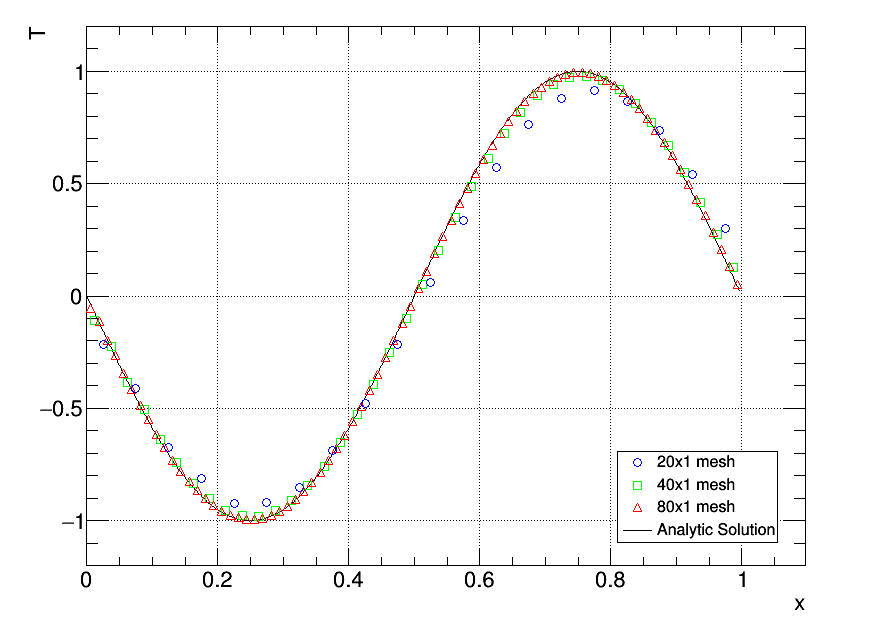
\includegraphics[width=0.85\linewidth]{qq11}
\caption{The solution at $t=1$ for mesh sizes of 20, 40, and 80}
\label{q4}
\end{figure}

The order of accuracy for the scheme was determined using the log log method as displayed in figure \ref{ord}. The order of accuracy for this scheme was estimated to be 2nd order accurate based on the $L_2$ data from 6 different meshes. This matches what was expect by implementing a 2nd order interior and boundary flux evaluation scheme. It should be noted as seen in figure \ref{qq22} the relative error decreases when refining the mesh. This is expect as the numerical solution is a discrete representation of the continuous exact solution.

 \begin{table}[H]
\begin{center}
    \begin{tabular}{ | p{0.13\linewidth} | p{0.2\linewidth} |p{0.1\linewidth} |p{0.1\linewidth} |p{0.1\linewidth} |}
 \hline  
     \RaggedRight \textbf{Mesh Size}
    &\RaggedRight \textbf{$L^2$norm}
    &\RaggedRight \textbf{$\triangle x$}
    &\RaggedRight \textbf{$\triangle t$}
    &\RaggedRight \textbf{Order}
    \\ \hline  
           \RaggedRight 20 x 1
    &\RaggedRight 8.158$*10^{-2}$
    &\RaggedRight 0.05
    &\RaggedRight 0.01
    &\RaggedRight -
    \\ \hline 
           \RaggedRight 40 x 1
    &\RaggedRight 2.399$*10^{-2}$
    &\RaggedRight 0.025
    &\RaggedRight 0.005
    &\RaggedRight 1.934
    \\ \hline 
           \RaggedRight 80 x 1
    &\RaggedRight 6.445$*10^{-3}$
    &\RaggedRight 0.0125
    &\RaggedRight 0.0025
    &\RaggedRight 1.937
    \\ \hline 
           \RaggedRight 160 x 1
    &\RaggedRight 1.676$*10^{-3}$
    &\RaggedRight 0.00625
    &\RaggedRight 0.00125
    &\RaggedRight 1.942
    \\ \hline 
 
    
    
    \end{tabular}
\end{center} 
\caption{Table of $L^2$ norms for increasing mesh size for $CFL = 0.4$}
\label{norm} 
\end{table}



\begin{figure}[H]
\centering
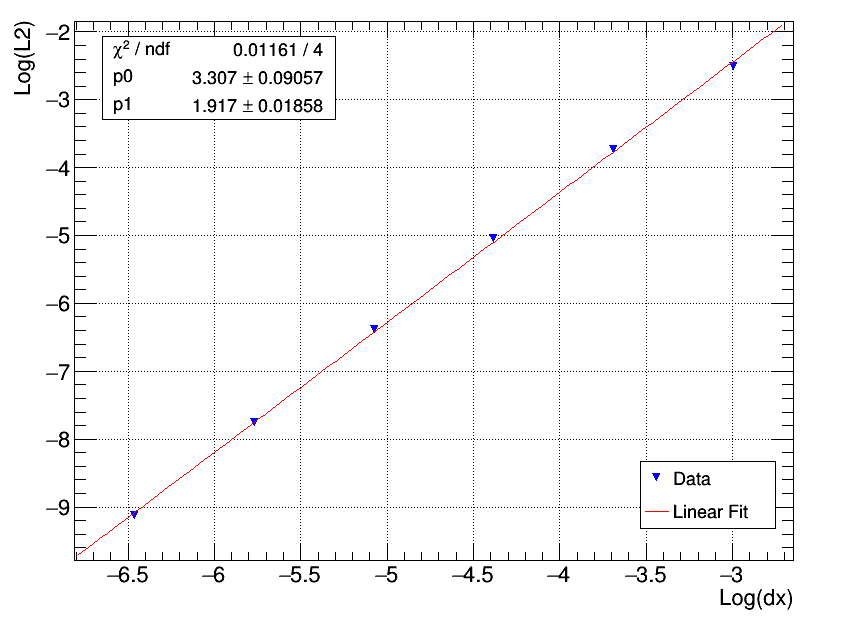
\includegraphics[width=0.85\linewidth]{order}
\caption{Calculated Order of Accuracy}
\label{ord}
\end{figure}

\begin{figure}[H]
\centering
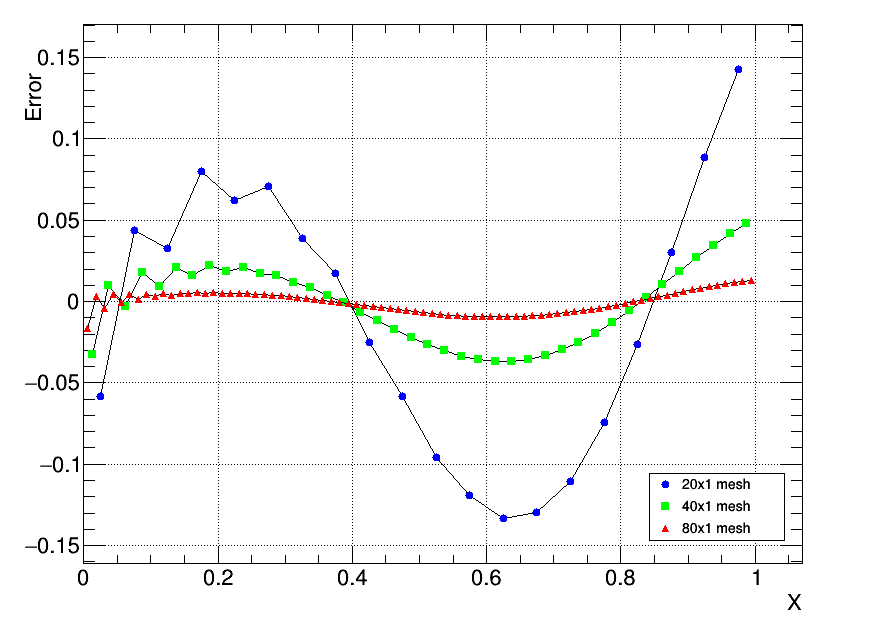
\includegraphics[width=0.85\linewidth]{qq22}
\caption{Solution Error at $t=1$ for mesh sizes of 20, 40, and 80}
\label{3D}
\end{figure}


The log-log plot enables us to estimate what mesh size would be required for a particular error. Extrapolating the plot it was found in order to obtain an error less than $10^{-3}$ a mesh size of 206.12 or greater is required. Similarly to obtain an error less than $10^{-4}$ a mesh of greater than 685.14 is required using a CFL number of 0.4. When determining what level of refinement should be used for a problem both the level of error mitigation and performance expenses should be considered.

\subsection{Stability}
Stability is an important factor when considering time advance schemes. Ideally one would like to advance to the required time solution in as few time steps as possible to reduce computation load. However if the time step is too large instabilities can arise causing the solution error to diverge exponentially. These can arise from the time dependent boundary, with a large time step the next solution change is calculate from a large boundary change which results in a large solution overshoot. The problem  compounds with the large overshoot as again the solution and time step boundary are vastly different. The stability limits of the program were experimentally determined by evaluating the $L_2$ norm as a function of increasing CFL number. A small CFL number corresponds to a small time step, therefore the $L_2$ norm was calculated relatively against an ideal stable time step. 



\begin{figure}[H]
\centering
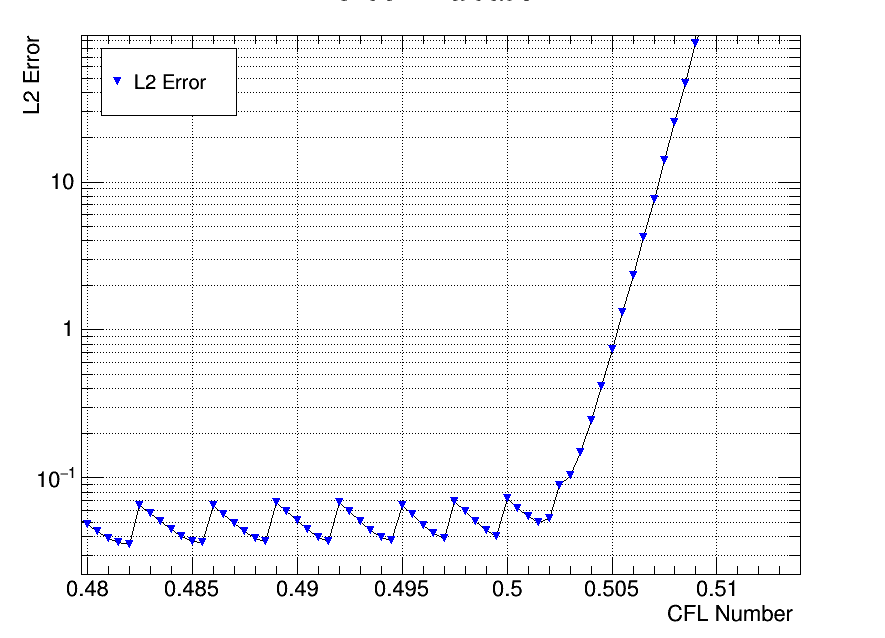
\includegraphics[width=0.85\linewidth]{stabl2}
\caption{The L2 error for increasing CFL number for a 500x1 mesh with $x_{max} = 20$}
\label{stbl1}
\end{figure}

The domain was extended to $x_{max} =20$ with the first section ($0\leq x \leq 1 $) is set as $-x$ and 0 everywhere else as initial conditions. The solution was computed at t=8 on a mesh of 500 control volumes. Figure \ref{stbl1} displays the $L_2$ norm error as a function of CFL near the instability regime. The plot identifies when the scheme becomes violently unstable in which case the solution is not a good representation of the exact solution. The maximum stable CFL was determined to be $0.500 \pm 0.005$. Anything above the value is considered slightly unstable or completely unstable.   

\begin{figure}[H]
        \centering
        \begin{subfigure}[h]{\textwidth}
                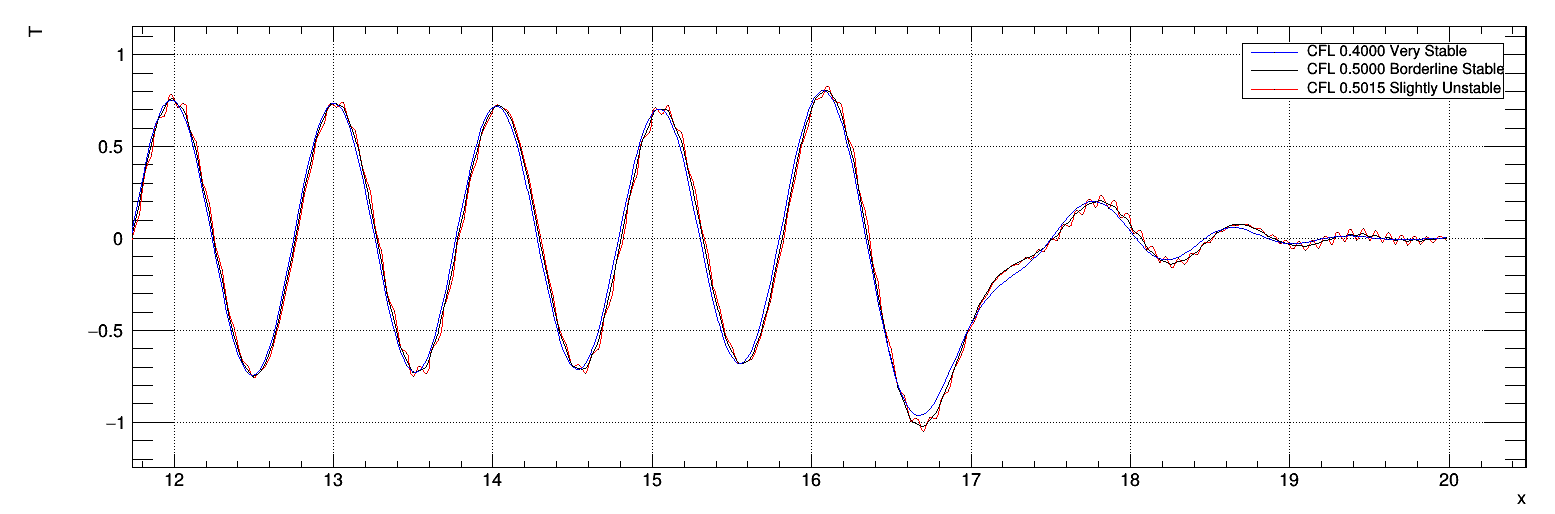
\includegraphics[width = 14.95cm]{stab1}
                \caption{}
				
        \end{subfigure}%
       ~~~~~
       
        \begin{subfigure}[h]{\textwidth}
                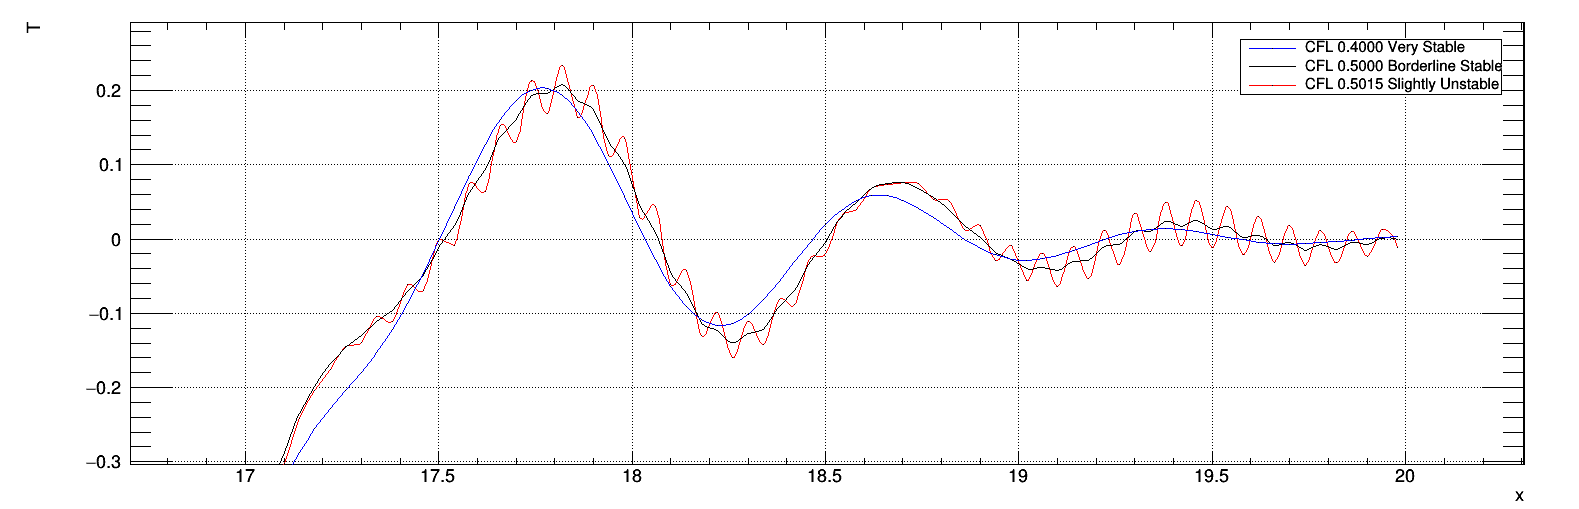
\includegraphics[width = 15.15cm]{stab3}
                \caption{}
                
        \end{subfigure}
        
        
        \begin{subfigure}[h]{\textwidth}
                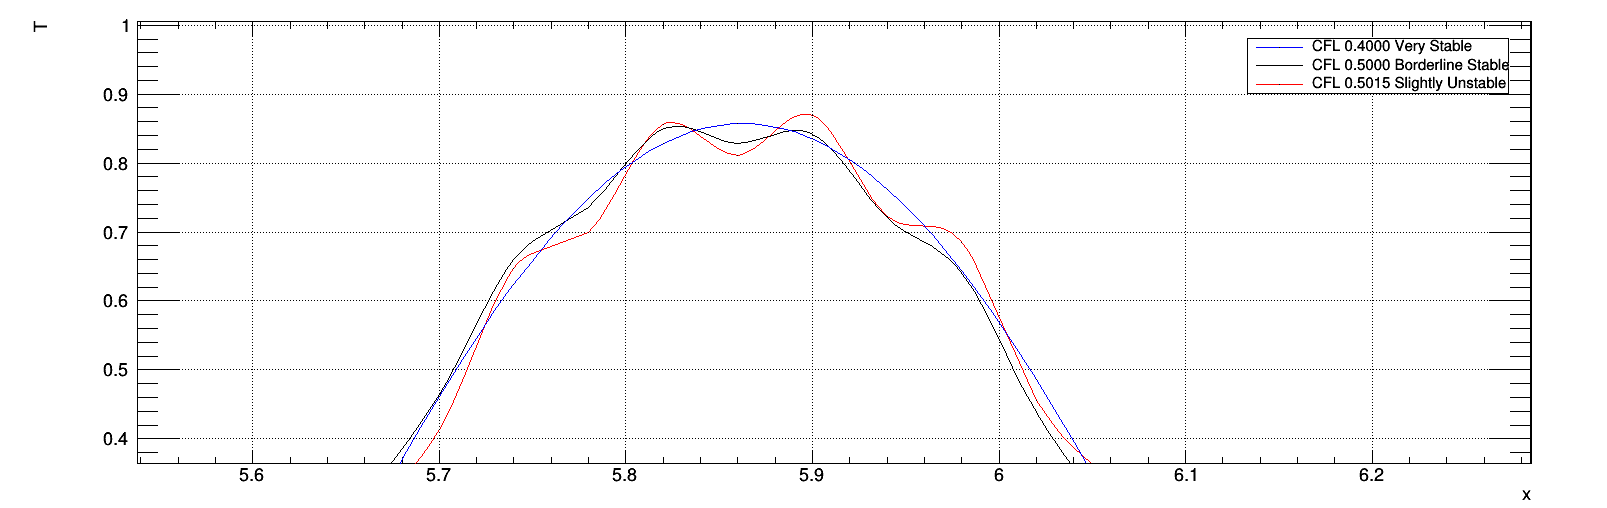
\includegraphics[width = 15.35cm]{stab2}
                \caption{}
                
        \end{subfigure}
        \caption{Comparison between a stable(blue), borderline (black) stable and slightly unstable (red) solution at $t=8$ for 500 control volumes}
        \label{q34}
\end{figure}

Figure \ref{q34} displays the visible differences between a stable, borderline stable and slightly unstable solution. Figure \ref{q34} part a) displays a zoomed out version of the solution. Only the slightly unstable solution has a visible difference. The instability is seen as the higher frequency oscillations developing about the path of the solution. As we zoom in further we can begin to see the board-line stable solution which appeared stable also contains some oscillatory characteristics in certain regions. These features grow exponentially with a further increase in CFL. It should be noted these features begin to appear at the same time the error begins to diverge, providing a simple means of determining the stability boundary of the solution. From theory we see the stability region is dependent on both the stability bounds of the 2nd order upwind method and the RK2 method. The 2nd upwind stability region is a circle with radius of $\frac{2u\triangle t}{\triangle x}$, while the RK2 is denoted as a approx circle of radius 1 (on real axis). Setting these equal and rearranging we find the theoretical CFL to be $0.5$ therefore CFL values between 0 and 0.5 should be stable. Comparing Experimental and theoretical values of max CFL for determining stability we find they are indeed consistent.

\subsection{Effect of Boundary Conditions}
Initial and boundary conditions are the parameters that differentiate a problem from its general form. Failure to setup or apply appropriate boundary conditions means you are solving a different problem which is going to give you the wrong solution. In addition to applying the correct boundary there are different methods for implying the same boundary, these methods however are not all created equal. The trade off is usually split between implementation and error mitigation. Complicated schemes usually reduce error, but sometimes can be at the price of performance or maintenance. Boundary condition methods should be closely investigated and tailored to the problem at hand. 

\begin{figure}[H]
\centering
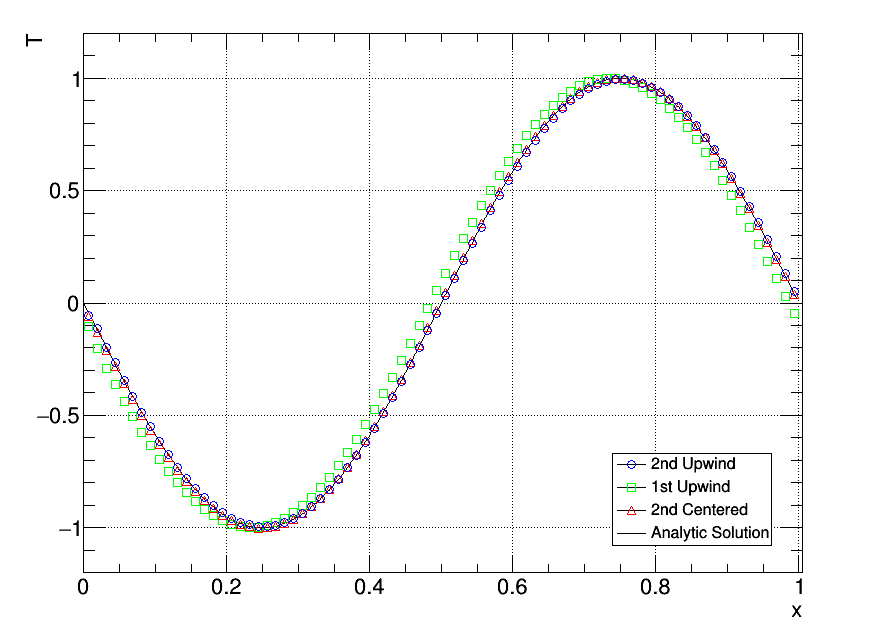
\includegraphics[width=0.75\linewidth]{3a1}
\caption{Displays Solution for 2nd Upwind, 1st Upwind and 2nd Centered schemes at $t=1$ for 80x1 mesh}
\label{3a1}
\end{figure}
For the wave equation three types of boundaries were implemented and compared to highlight their strengths and weaknesses. In addition to the 2nd order upwind (2UW) boundary implementation used in the previous sections a 1st order upwind (1UW) and 2nd order centered (2CE) scheme were investigated for mesh of 80x1 for a CFL of 0.4 where $x_{max} = 1.0$. It should be noted the interior scheme remains 2nd order upwind. The solution implementing each boundary condition is plotted in \ref{3a1} and the relative error against the exact solution in \ref{3a2}.

\begin{figure}[H]
\centering
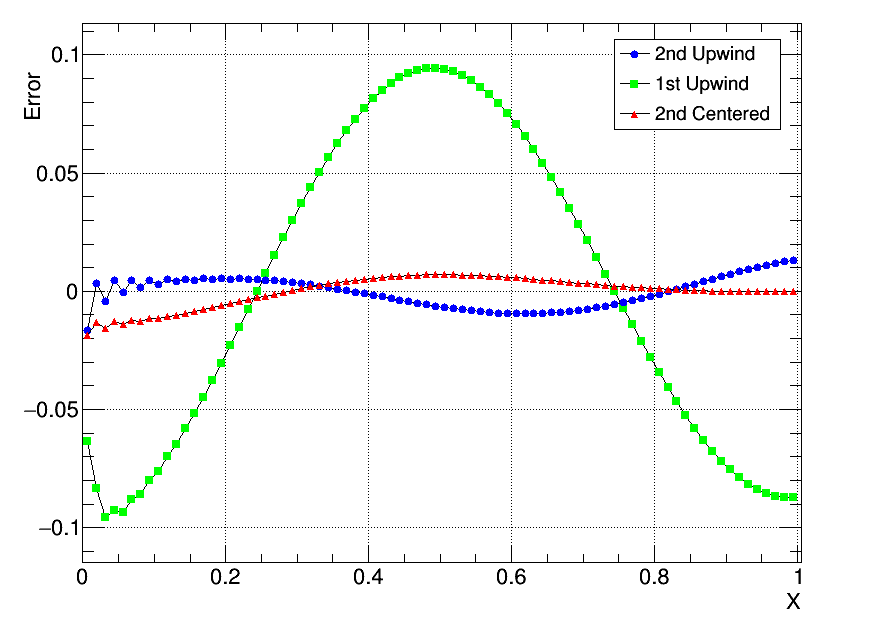
\includegraphics[width=0.75\linewidth]{3a2}
\caption{Solution Error for 2nd Upwind, 1st Upwind and 2nd Centered schemes at $t=1$ for 80x1 mesh}
\label{3a2}
\end{figure}

The difference between a second and 1st order scheme is immediately apparent in the relative error comparison. From this plot (figure \ref{3a2} there are little differences between the 2UW and 2CE. They both appear to have the same level of error just opposite overshoots. In order to gain beter understanding of the error behavior between the three schemes the $L_1$ and $L_{\infty}$ were plotted against mesh size for each as shown in figure \ref{3a3}.

\begin{figure}[H]
\centering
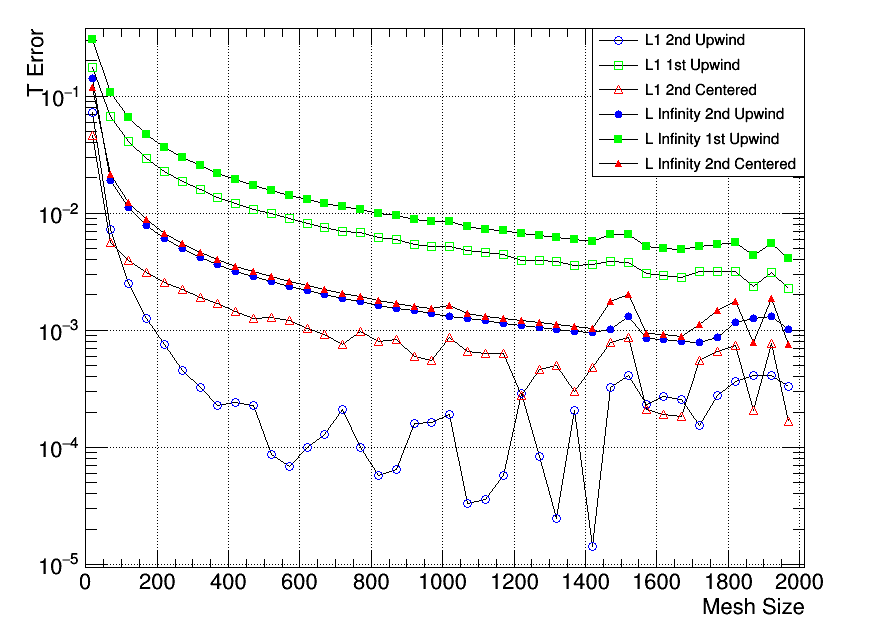
\includegraphics[width=0.75\linewidth]{3a33}
\caption{The $L_1$ and $L_{\infty}$ relative mesh size refinement for 2UW, 1UW and 2CE schemes}
\label{3a3}
\end{figure}

Its immediately apparent that the error for 2nd order schemes converges must faster than the 1st order method and is reduce by almost an order of magnitude. Its interesting to note how profound the effect of boundaries have on the solution. For example considered the 1UW scheme, though the entire interior domain uses a 2nd order scheme, using a 1st order boundary scheme is enough to render the entire solution to basically 1st order accuracy. The 2UW scheme seems to produce the lowest errors across the board however comes at the expense of 2 extra ghost cells. For large grid problems this can be expensive in terms of memory and efficiency. Now for each iteration two extra rows needs to be evaluated at each boundary, for grids with millions of cells this would be expensive processing wise. However this may be traded off by the fact the interior scheme can be applied unaltered to the bordering cell volumes. The 2CE could be competitive in the sense it does not require as many or any additional cells for boundary evaluation. Its clear the boundaries have a profound effect on the solution error and should be the first consideration in any large CFD problem.

\section{Conclusion}
This project provides great insight into the internal algorithms used for calculating numerical solutions for time varying problems. The Wave Equation problem provided a great platform for developing and testing the program. Having the analytic solution really help fine tune the program and helped given an idea on how accurate the solutions could be. Investigating the error and how it changes relative to boundaries and mesh sizes will provides insight on how the methods should be applied to bigger problems to minimize time and error. Stability analysis provided a great means for understanding the computational limits of the program in terms of speed. Numerical methods provide a great way of solving difficult problems and until new methods are discovered for finding exact solution will remain the main method for finding solutions to difficult problems. 






\appendix
\section{Appendix} \label{App:Appendix}
\subsection{wave.cpp}
\begin{lstlisting}
/*-------------------------------------------------------------------------------//
Main Program for finding solutions for wave equation. Employs a RK2 time advance 
with 2nd order upwind flux scheme.


Jerin Roberts 2016
compiled using g++/gcc version 5.4.0 on Ubuntu 16.04.02 and are available for clone 
via the link provided: url{https://github.com/j16out/
//-------------------------------------------------------------------------------*/


#include <vector>
#include <iostream>
#include <cstdlib>
#include <fstream>
#include <string>
#include <vector>
#include <algorithm>
#include <sstream>
#include <math.h> 
#include "TApplication.h"
#include "vroot/root.hpp"
#include "numerical/numerical.hpp"

using namespace std;




int main(int argc, char **argv)
{


carray wave1;//my main array
carray analytic1;
carray wave2;//my main array
carray analytic2;
carray wave3;//my main array
carray analytic3;
carray wave4;//my main array
carray analytic4;
carray wave5;//my main array
carray analytic5;
carray wave6;//my main array
carray analytic6;


//set size


//set array size or default used 162x162
set_array_size(wave1, 20, 1, 1.0, 0);//array, xsize, ysize, dimension
set_array_size(wave2, 40, 1, 1.0, 0);
set_array_size(wave3, 80, 1, 1.0, 0);
set_array_size(wave4, 160, 1, 1.0, 0);//array, xsize, ysize, dimension
set_array_size(wave5, 320, 1, 1.0, 0);
set_array_size(wave6, 686, 1, 1.0, 0);

set_array_size(analytic1, 20, 1, 1.0, 0);
set_array_size(analytic2, 40, 1, 1.0, 0);
set_array_size(analytic3, 80, 1, 1.0, 0);
set_array_size(analytic4, 160, 1, 1.0, 0);
set_array_size(analytic5, 320, 1, 1.0, 0);
set_array_size(analytic6, 686, 1, 1.0, 0);




//print_array(analytic);



//set intial conditions


set_zero(wave1);
set_intial_cond(wave1);
//print_array(wave1);//print array in terminal
set_zero(wave2);
set_intial_cond(wave2);

set_zero(wave3);
set_intial_cond(wave3);

set_zero(wave4);
set_intial_cond(wave4);
//print_array(wave1);//print array in terminal
set_zero(wave5);
set_intial_cond(wave5);

set_zero(wave6);
set_intial_cond(wave6);



float l2 = 0;

//---------------------solve array1----------------------//
solve_arrayRK2(wave1, 1.0, 0.4);//array,time,cfl
set_analytic(analytic1, wave1);
l2 = get_l2norm(wave1, analytic1);
wave1.l2norm.push_back(l2);
//cout << "Solution: " << get_solution(poisson1) << "\n";



//---------------------solve array2----------------------//
solve_arrayRK2(wave2, 1.0, 0.4);
set_analytic(analytic2, wave2);
l2 = get_l2norm(wave2, analytic2);
wave1.l2norm.push_back(l2);


//---------------------solve array2----------------------//
solve_arrayRK2(wave3, 1.0, 0.4);
set_analytic(analytic3, wave3);
l2 = get_l2norm(wave3, analytic3);
wave1.l2norm.push_back(l2);

//---------------------solve array1----------------------//
solve_arrayRK2(wave4, 1.0, 0.4);//array,time,cfl
set_analytic(analytic4, wave4);
l2 = get_l2norm(wave4, analytic4);
wave1.l2norm.push_back(l2);
//cout << "Solution: " << get_solution(poisson1) << "\n";



//---------------------solve array2----------------------//
solve_arrayRK2(wave5, 1.0, 0.4);
set_analytic(analytic5, wave5);
l2 = get_l2norm(wave5, analytic5);
wave1.l2norm.push_back(l2);


//---------------------solve array2----------------------//
solve_arrayRK2(wave6, 1.0, 0.4);
set_analytic(analytic6, wave6);
l2 = get_l2norm(wave6, analytic6);
wave1.l2norm.push_back(l2);



//----------------------Draw Data---------------------//

if(1)//start root application
{
	TApplication theApp("App", &argc, argv);//no more than two subs 
	draw_graph_q1(wave1, wave2, wave3, analytic1, analytic2, analytic3);   
	theApp.Run();
}

 //draw_graph_wave1(wave1, wave2, wave3);


//end
}

\end{lstlisting}
\subsection{numerical.hpp}
\begin{lstlisting}
#ifndef numerical_INCLUDED
#define numerical_INCLUDED


#include <vector>
#include <iostream>
#include <cstdlib>
#include <fstream>
#include <string>
#include <vector>
#include <algorithm>
#include <sstream>
#include <math.h> 
#include <iomanip>

using namespace std;

#define BIG 10000
#define maxx 8000
#define maxy 3
#define PI 3.141592654



struct carray{
//arrays
float mcellSOL [maxx][maxy];//first stage and solution mesh
float mcellSOL2 [maxx][maxy];//second stage solution mesh
float mcellFI [maxx][maxy];//first stage flux
float mcellFI2 [maxx][maxy];//second stage flux

//array attributes
int sizex = maxx;
int sizey = maxy;
float DIM1 = 0;

//current time 
float tstep = 0;
float ctime = 0;

//data storage specific to array
vector<float> l2norm;
vector<float> l1norm;
vector<float> linfnorm;
vector<float> diff;

//temporary cells to store
float Tim2_j=0.0;
float Tim1_j=0.0;
float Ti_j=0.0;
float Tip1_j=0.0;

//scheme
int scheme = 0;

};

//--------------------Init Arrays-----------------------------------------//

void set_array_size(carray & myarray, int x, int y, float DIM, int scheme);//set array size

void set_zero(carray & myarray);//zero entire array

void print_array(carray & myarray);//print array in terminal



//-------------------Boundary and Intial Conditions------------------------//

void set_ghostcells(carray & myarray);//set ghost cells

void set_intial_cond(carray & myarray);

void set_intial_cond2(carray & myarray);

//--------------------RK2 solver functions----------------------------------//

void get_FIarray(carray & myarray, int stage);//get all FI for array for specific stage

void get_FIarray_1stcell(carray & myarray, int stage);

void get_surcells(carray & myarray, int i, int j, int stage);//obtain values of surrounding cells stage defines were result stored

void get_RK2(carray & myarray, int stage);

void mv_SOL2_to_SOL1(carray & myarray);

void solve_arrayRK2(carray & myarray, float tmax, float cfl);//solve the array

//flux schemes
float calc_2nd_UW(carray & myarray);//calculate new cell value based on 2nd order scheme
float calc_1st_UW(carray & myarray);
float calc_2nd_CE(carray & myarray);


//-----------------------Error calc related functions---------------------------//

float get_l2norm(carray & myarray, carray myarray2);//get estimated vale for l2 norm between arrays
float get_linf_norm(carray & myarray, carray myarray2);
float get_l1norm(carray & myarray, carray myarray2);

void set_analytic(carray & myarray, carray & numarray);//set analytic solution to a mesh



#endif

\end{lstlisting}
\subsection{numerical.cpp}
\begin{lstlisting}
#include "numerical.hpp"





//**************************************************************************//
//---------------------------Setting Array----------------------------------//
//**************************************************************************//


//----------set array size (working area excluding ghost)---------------//

void set_array_size(carray & myarray, int x, int y, float DIM, int scheme)
{
	if(x <= 8000 && y <= 3)
	{
	myarray.sizex = x+2;
	myarray.sizey = y+2;
	myarray.DIM1 = DIM/(x);
	myarray.scheme = scheme;
	}
	else
	cout << "Array size to big, setting to default 160" << "\n";

}

//--------------------------Print array in terminal----------------------------//

void print_array(carray & myarray)
{
cout << "\n";

	for(int j = 0; j < myarray.sizey; ++j)
	{
	cout << "\n|";	
		for(int i = 0; i < myarray.sizex; ++i)
		{
		if(myarray.mcellSOL[i][j] >= 0)
		cout << setprecision(3) << fixed << myarray.mcellSOL[i][j] <<"|";
		if(myarray.mcellSOL[i][j] < 0)
		cout << setprecision(2) << fixed << myarray.mcellSOL[i][j] <<"|";
		}
	
	}
cout << "\n";
}


//--------------------------zero array----------------------------//

void set_zero(carray & myarray)
{
	for(int j = 0; j < myarray.sizey; ++j)
	{
		for(int i = 0; i < myarray.sizex; ++i)
		{
		myarray.mcellSOL[i][j] = 0;//set everything to zero
        myarray.mcellSOL2[i][j] = 0;
        myarray.mcellFI2[i][j] = 0;
        myarray.mcellFI[i][j] = 0;
		}
	}
}


//--------------------------set ghost cells for Wave----------------------------//


void set_ghostcells(carray & myarray)
{
float DIM1 = myarray.DIM1;

//set boundary conditions in ghost cells
if(myarray.scheme == 0)//2nd order upwind
{
myarray.mcellSOL2[0][1] = -2.0*(sin(4.0*PI*myarray.ctime)) + 3.0*myarray.mcellSOL[1][1];
myarray.mcellSOL2[1][1] = 2.0*(sin(4.0*PI*myarray.ctime)) - myarray.mcellSOL[2][1];
}

if(myarray.scheme == 1)//1st order upwind
{
myarray.mcellSOL2[1][1] = 2.0*(sin(4.0*PI*myarray.ctime)) - myarray.mcellSOL[2][1];
}

if(myarray.scheme == 2)//2nd order centered
{
myarray.mcellSOL2[1][1] = 2.0*(sin(4.0*PI*myarray.ctime)) - myarray.mcellSOL[2][1];
}


	
}

//--------------------------set intial condition---------------------------------//

void set_intial_cond(carray & myarray)
{
float DIM1 = myarray.DIM1;
float dx =0.0;
float f;

for(int j = 1; j < myarray.sizey-1; ++j)
{

    for(int i = 2; i < myarray.sizex; ++i)
    {
    dx = (i-1.5)*DIM1;
    f = -sin(2.0*PI*dx);
    myarray.mcellSOL[i][j] = f;
    //printf("f: %f  dx: %f\n", f, dx);
    }

}
}

void set_intial_cond2(carray & myarray)
{
float DIM1 = myarray.DIM1;
float dx =0.0;
float f;

for(int j = 1; j < myarray.sizey-1; ++j)
{

    for(int i = 2; i < myarray.sizex; ++i)
    {
    dx = (i-1.5)*DIM1;
    if(dx <= 1.0)
    {
    f = -dx;
    myarray.mcellSOL[i][j] = f;
    }
    else
    {
    f = 0.0;
    myarray.mcellSOL[i][j] = f;
    }
    //printf("f: %f  dx: %f\n", f, dx);
    }

}
}


//**************************************************************************//
//---------------------------RK2 Array Solving------------------------------//
//**************************************************************************//

//--------------------------Set FI values for array mcellFI Face----------------------------//

void get_FIarray_1stcell(carray & myarray, int stage)
{

int j = 1;
int i = 2;
float newcell;

//----get surrounding cells and compute new cell-------//
get_surcells(myarray, i, j, stage);
if(myarray.scheme == 0)
newcell = calc_2nd_UW(myarray); 

if(myarray.scheme == 1)
newcell = calc_1st_UW(myarray); 

if(myarray.scheme == 2)
newcell = calc_2nd_CE(myarray); 

//-----update current cell----//
if(stage == 1)
myarray.mcellFI[i][j] = newcell;

if(stage == 2)
myarray.mcellFI2[i][j] = newcell;

	

}

//--------------------------Set FI values for array mcellFI Interior----------------------------//

void get_FIarray(carray & myarray, int stage)
{


for(int j = 1; j < myarray.sizey-1; ++j)
{

    for(int i = 3; i < myarray.sizex; ++i)
    {

    //----get surrounding cells and compute new cell-------//
    get_surcells(myarray, i, j, stage);
    float newcell = calc_2nd_UW(myarray); 

    //-----update current cell----//
    if(stage == 1)
    myarray.mcellFI[i][j] = newcell;

    if(stage == 2)
    myarray.mcellFI2[i][j] = newcell;
    }

}
	

}


//--------------------Calculate new cell value from neighbors ---------------------//


float calc_2nd_UW(carray & myarray)
{
float DIM1 = myarray.DIM1;
float chx = DIM1;
//float chy = DIM1;
float temp = 1.0;
float newcell = (2.0)*(3.0*myarray.Ti_j-4.0*myarray.Tim1_j+myarray.Tim2_j)/(2.0*chx);

return newcell;
}


float calc_1st_UW(carray & myarray)
{
float DIM1 = myarray.DIM1;
float chx = DIM1;
//float chy = DIM1;
float temp = 1.0;
float newcell = (2.0)*(myarray.Ti_j-myarray.Tim1_j)/(2.0*chx);

return newcell;
}


float calc_2nd_CE(carray & myarray)
{
float DIM1 = myarray.DIM1;
float chx = DIM1;
//float chy = DIM1;
float temp = 1.0;
float newcell = (2.0)*(myarray.Tip1_j-myarray.Tim1_j)/(2.0*chx);

return newcell;
}




//--------------------------Get current cell values----------------------------//

void get_surcells(carray & myarray, int i, int j, int stage)
{
float fcon = false;
float sizex = myarray.sizex;
float sizey = myarray.sizey;

if(stage == 1)//get surrounding cell values
{
myarray.Tim1_j = myarray.mcellSOL[i-1][j];
myarray.Tim2_j = myarray.mcellSOL[i-2][j];
myarray.Ti_j = myarray.mcellSOL[i][j]; 
myarray.Tip1_j = myarray.mcellSOL[i+1][j];

} 

if(stage == 2)
{
myarray.Tim1_j = myarray.mcellSOL2[i-1][j];
myarray.Tim2_j = myarray.mcellSOL2[i-2][j];
myarray.Ti_j = myarray.mcellSOL2[i][j];
myarray.Tip1_j = myarray.mcellSOL[i+1][j];
 
} 
        

}

//-----------------------------cp array2 to 1---------------------------//

void mv_SOL2_to_SOL1(carray & myarray)
{

for(int j = 0; j < myarray.sizey; ++j)
{

    for(int i = 0; i < myarray.sizex; ++i)
    {
    myarray.mcellSOL[i][j] = myarray.mcellSOL2[i][j];//move update solution to array 1 
    }
}

}

//--------------------------Solve array using RK2 and 2ndUW----------------------------//

void solve_arrayRK2(carray & myarray, float tmax, float cfl)
{
int tomp;
float tstep = (cfl*(myarray.DIM1))/2.0;
myarray.tstep = tstep;
float ctime = myarray.ctime;
set_intial_cond(myarray);
set_ghostcells(myarray);

printf("\n\nRunning size: %d time step: %f\n",myarray.sizex,myarray.tstep);

int n = 0;
int nt = 1000;
while(ctime < tmax-tstep)
{

if(n >= nt)//status
{
printf("Run: %d time: %f\n",n,myarray.ctime);
nt = 1000+n;
}

//FI and RK2 for stage 1 and 2
    for(int h = 1; h <= 2; ++h)
    { 
    get_FIarray_1stcell(myarray, h);//(array, stage)
    get_FIarray(myarray, h);
    get_RK2(myarray, h);
    }
//flux at boundary
set_ghostcells(myarray);

//mv sol2 back to array sol1
mv_SOL2_to_SOL1(myarray);

//advance and record time steps
myarray.ctime = myarray.ctime+myarray.tstep;
ctime = myarray.ctime;
++n;
}

printf("Solved numeric at %f time\n",ctime);
}

//--------------------------Solve RK2 interation----------------------------//


void get_RK2(carray & myarray, int stage)
{

if(stage == 1)//first stage RK2
{
for(int j = 1; j < myarray.sizey-1; ++j)
{

    for(int i = 2; i < myarray.sizex; ++i)
    {
      myarray.mcellSOL2[i][j] = myarray.mcellSOL[i][j]-myarray.tstep*(myarray.mcellFI[i][j]);
    }

}
}

if(stage == 2)//second stage RK2
{
for(int j = 1; j < myarray.sizey-1; ++j)
{

    for(int i = 2; i < myarray.sizex; ++i)
    {
     myarray.mcellSOL2[i][j] = myarray.mcellSOL[i][j]-myarray.tstep*((myarray.mcellFI2[i][j]+myarray.mcellFI[i][j])/2.0);
    }

}
}



}



//**************************************************************************//
//---------------------------Error Checking---------------------------------//
//**************************************************************************//





//-------------------------Get L1 norm for unknown analytical----------------------//

float get_l1norm(carray & myarray, carray myarray2)
{
float l1sum =0;
float sx = myarray.sizex-2;
float sy = myarray.sizey-2;

for(int j = 1; j < myarray.sizey-1; ++j)
{	
	for(int i = 2; i < myarray.sizex; ++i)
	{

	float P = myarray.mcellSOL[i][j];
	float T = myarray2.mcellSOL[i][j];
	l1sum =  l1sum + abs(P-T);

	}

}

float l1 = l1sum/(sx);
cout << setprecision(8) << fixed << "L1 norm: " << l1 << "\n";
return l1;
}


//-------------------------Get L infinty norm for unknown analytical----------------------//

float get_linf_norm(carray & myarray, carray myarray2)
{
float error =0;
float maxerror = -1;
float sx = myarray.sizex-2;
float sy = myarray.sizey-2;

for(int j = 1; j < myarray.sizey-1; ++j)
{	
	for(int i = 2; i < myarray.sizex; ++i)
	{

	float P = myarray.mcellSOL[i][j];
	float T = myarray2.mcellSOL[i][j];
	error =  abs(P-T);
    if(error > maxerror)
    maxerror = error;

	}

}


cout << setprecision(8) << fixed << "L infinity norm: " << maxerror << "\n";
return maxerror;
}



//-------------------------Get L2 nrom for unknown analytical----------------------//

float get_l2norm(carray & myarray, carray myarray2)
{
float l2sum =0;
float sx = myarray.sizex-2;
float sy = myarray.sizey-2;

for(int j = 1; j < myarray.sizey-1; ++j)
{	
	for(int i = 2; i < myarray.sizex; ++i)
	{

	float P = myarray.mcellSOL[i][j];
	float T = myarray2.mcellSOL[i][j];
	l2sum =  l2sum + pow((P-T),2);

	}

}

float l2 = sqrt(l2sum/(sx));
cout << setprecision(8) << fixed << "L2 norm: " << l2 << "\n";
return l2;
}



//----------------------------Set a Analytical Solution------------------------------//
void set_analytic(carray & myarray, carray & numarray)
{
float DIM1 = myarray.DIM1;
float ctime = numarray.ctime;
for(int j = 1; j < myarray.sizey-1; ++j)
{

	for(int i = 2; i < myarray.sizex; ++i)
	{
	float dx = (i-1.5)*DIM1;
	float dy = (j-1.5)*DIM1;
	float T = sin(2*PI*(2*(ctime)-dx));
	myarray.mcellSOL[i][j] = T;
	}

}

printf("setting analytic at %f time\n",ctime);
}


\end{lstlisting}

\begin{thebibliography}{99} % Beamer does not support BibTeX so references must be inserted manually as below
\bibitem[Celik, 2006]{p0}Ismail B. Celik1, Urmila Ghia, Patrick J.Roache and Christopher J. Freitas
\newblock "Procedure for Esitmation and Reporting Uncertainty Due to Discretization in CFD apllications",  West Virginia University, Morgantown WV, USA

\end{thebibliography}


%%% End document
\end{document}